\label{supp:exp}

\subsection{Estimating the Q Function}
\label{supp:sub:sub:q}
In Section \ref{sec:algorithm} we briefly discussed the possibility of avoiding explicitly estimating the Q function.  All the terms in \eqref{equ:expert-gradient} can be computed directly, with the exception of the Q function.  One approach therefore is to train an additional function approximator targeting the Q function directly.  This can then be used to estimate the discounted sum of rewards ahead given a particular action and belief state (when $\beta = 0$) without directly using the Monte Carlo rollouts.  However, estimating the Q function increases the computational cost, increases the number of hyperparameters that need tuning, and can lead to instabilities and biased training by over reliance on imperfect function approximators, especially in high-dimensional environments.  Therefore, as in many on-policy RL algorithms, an alternative is to use Monte Carlo estimates of the Q function, computed directly from a sampled trajectory (c.f. \eqref{equ:a2d:a2d_update}-\eqref{equ:a2d:gae}).  

However, somewhat unexpectedly, this second approach can lead to the systemic failure of A2D in particular \emph{environments}.  This can be shown by expanding the definition of $Q^{{\pi_{\psi}}}(a,b)$:
\begin{align}
     Q^{{\pi_{\psi}}}(a,b) = \mathop{\mathbb{E}}_{p(s, s'|a,b)} \Bigg[ \mathop{\mathbb{E}}_{d^{{\pi_{\psi}}}(b'|s')} \Big[ r(s,a,s') + \mathop{\gamma\mathbb{E}}_{\pi_{\psi}(a'|b')} \left[ Q^{\pi_{\psi}} (a', b') \right] \Big] \Bigg], \label{supp:equ:q_loss}
\end{align}
where $s'$ and $b'$ are the state and belief state after taking action $a$ in state $s$ and belief state $b$.  Since sampling from $p(s, s'|a,b)$ and $d^{{\pi_{\psi}}}(b' | s')$ is intractable, directly using the trajectories is equivalent to using a singled sample value throughout this expression \emph{and} the gradient estimator in \eqref{equ:a2d:a2d_update}.  Re-using just a single value of $s$ inside and outside of this expectation biases the gradient estimator, as the estimate of $Q$ is \emph{not} conditionally independent of the current (unobserved) state given the belief state.  Intuitively, using Monte Carlo rollouts  essentially allows the expert to ``cheat'' by learning using exclusively the true state and reward signal over a \emph{single} time step of a trajectory.  

When the Q function is estimated directly, the expectation in \eqref{supp:equ:q_loss} is estimated directly by the learned Q function, thereby amortizing this inference by learning across many different sampled trajectories.  Therefore, from a theoretical perspective, estimating the Q function is important for A2D to be guaranteed to function.  However, we find that this bias is only significant in specific environments, and hence, in many environments, explicitly estimating the Q function can be avoided.  This reduces the computational cost of the algorithm, and reduces the number of hyperparameters and network architectures that need tuning.  Furthermore, and most importantly, this eliminates the direct dependence on faithfully approximating the Q function, which, in environments with high-dimensional observations and actions, can be prohibitively difficult.  

To explore this behavior, and verify this theoretical insight, we introduce three variants of the Tiger Door problem, shown in Figure \ref{supp:fig:grid:OSC}.  The first variant, ``Tiger Door 1,'' shown in Figure \ref{supp:fig:grid:OSC:td1}, actually corresponds to a gridworld embedding of the original Tiger Door problem~\citep{littman1995pomdp}.  ``Tiger Door 2'' \& ``Tiger Door 3,'' shown in Figures \ref{supp:fig:grid:OSC:td2} and \ref{supp:fig:grid:OSC:td3}, then separate the goal by one and two squares respectively.  

The analysis above predicts that A2D should not be able to solve Tiger Door 1 without direct estimation of the Q function.  This is because the expert can reach the goal with certainty in a single action, which ends the episode.  This means the expert can always maximize reward by proceeding directly to the goal, and as the episode ends, the gradient signal is dominated by the bias from the single step.  This causes the expert to put additional mass on directly proceeding to the goal, even though the goal is not visible to the agent.  We note that this is also the most extreme example of this bias, and we believe this environment to be somewhat of an unusual corner-case.  

However, in Tiger Doors 2 and 3, the episode does not end immediately after proceeding directly towards the goal.  Therefore, the value of proceeding directly towards the goal is diminished, as the marginalization over state provided by GAE and the value function reduces the estimated advantage value.  The gradient computed in these scenarios is therefore dramatically less biased, to the point where directly estimating the Q function not required.  

The predicted behavior is indeed observed when applying A2D to each Tiger Door variant, shown in Figure \ref{supp:fig:grid:OSC}.  We see that in Tiger Door 1, the correct policy is only recovered when the Q function is explicitly estimated.  When the Q function is not estimated, the expert directly optimizes just the reward under the MDP, earning itself a reward of $18$, but rendering an implicit policy that performs poorly, earning a reward of $-42$.  In Tiger Doors 2 \& 3, the correct trainee policy is recovered regardless of whether a Q function is explicitly learned.  Interestingly, we observe that the policy divergence, $F(\psi)$, is often lower during training when using the Q function.  This further reinforces that estimating the Q function more directly optimizes the reward of the trainee.  We note, however, that the \emph{final} divergence achieved by the Q function is often higher than that obtained without Q. This is likely due to the systemic bias introduced by using function approximation.  Note that for all of these experiments we use the compact representation.  

\begin{figure}[t]

    \begin{subfigure}[t]{0.3\textwidth}
        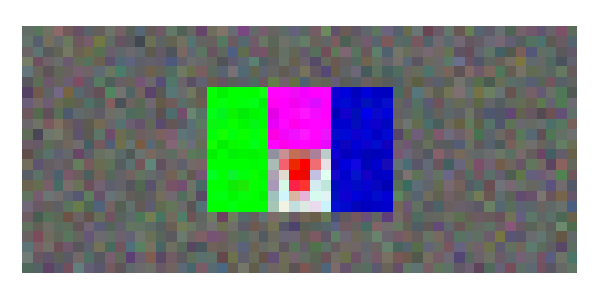
\includegraphics[width=\textwidth]{figures/OSC/TD1.pdf}
        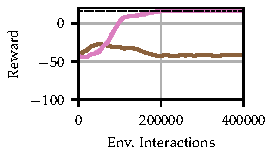
\includegraphics[width=\textwidth]{figures/OSC/cr_osc_6/OSC_TD1_lam05_reward_TigerDoor_True_v1_cr_osc_6_q0_2021_06_07__23_18_14_.pdf}
        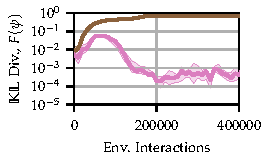
\includegraphics[width=\textwidth]{figures/OSC/cr_osc_6/OSC_TD1_lam05_divergence_TigerDoor_True_v1_cr_osc_6_q0_2021_06_07__23_18_14_.pdf}
        \caption{Tiger Door 1.}
        \label{supp:fig:grid:OSC:td1}
    \end{subfigure}%
    %
    \hfill%
    %
    \begin{subfigure}[t]{0.3\textwidth}
        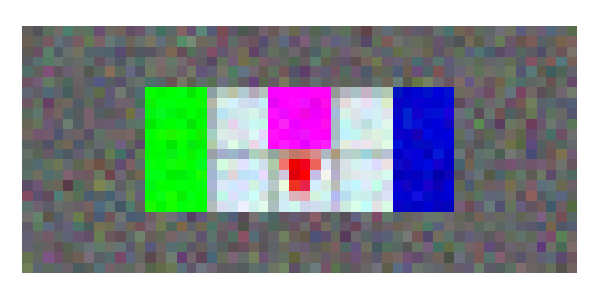
\includegraphics[width=\textwidth]{figures/OSC/TD2.pdf}
        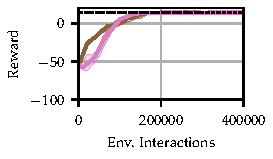
\includegraphics[width=\textwidth]{figures/OSC/cr_osc_6/OSC_TD2_lam05_reward_TigerDoor_True_v2_cr_osc_6_q0_2021_06_07__18_05_38_.pdf}
        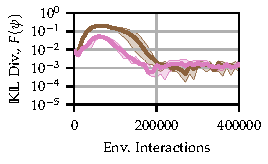
\includegraphics[width=\textwidth]{figures/OSC/cr_osc_6/OSC_TD2_lam05_divergence_TigerDoor_True_v2_cr_osc_6_q0_2021_06_07__18_05_38_.pdf}
        \caption{Tiger Door 2.}
        \label{supp:fig:grid:OSC:td2}
    \end{subfigure}%
    %
    \hfill%
    %
    \begin{subfigure}[t]{0.3\textwidth}
        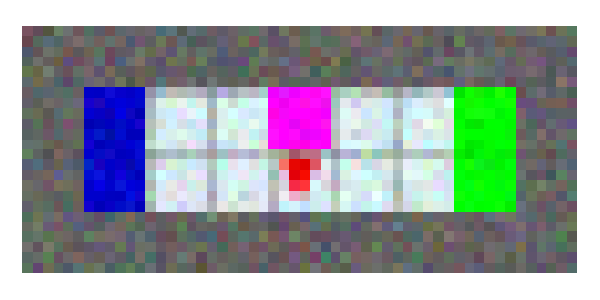
\includegraphics[width=\textwidth]{figures/OSC/TD3.pdf}
        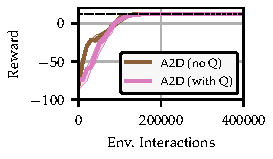
\includegraphics[width=\textwidth]{figures/OSC/cr_osc_6/OSC_TD3_lam05_reward_TigerDoor_True_v3_cr_osc_6_q0_2021_06_07__18_05_38_.pdf}
        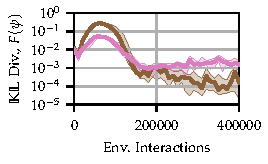
\includegraphics[width=\textwidth]{figures/OSC/cr_osc_6/OSC_TD3_lam05_divergence_TigerDoor_True_v3_cr_osc_6_q0_2021_06_07__18_05_38_.pdf}
        \caption{Tiger Door 3.}
        \label{supp:fig:grid:OSC:td3}
    \end{subfigure}%

    \caption{Results investigating requirement of directly estimating the Q function, as initially introduced in Section \ref{sec:algorithm} and discussed further in Section \ref{supp:sub:sub:q}.  Median and quartiles across $20$ random seeds are shown.  The Q function is learned targeting the expected discounted sum of rewards ahead conditioned on a particular (belief) state-action pair.  A value function is also learned in this way, and is used in conjunction with the Q function to directly estimate the advantage in \eqref{equ:a2d:a2d_update}.  Hence the A2D gradient is computed without direct use of Monte Carlo rollouts.  When no Q function is being used, the advantage is computed using GAE (c.f. Equations \eqref{equ:a2d:a2d_update}-\eqref{equ:a2d:gae}), with $\lambda = 0.5$.  We instantly anneal $\beta = 0$.  { }%  
    %
    Figure \ref{supp:fig:grid:OSC:td1}: Training curves for Tiger Door 1~\citep{littman1995pomdp}.  As predicted by the discussion in Section \ref{supp:sub:sub:q}, A2D does not converge to the correct policy if a Q function is not simultaneously learned.  This deficiency is instrumented by the high $\mathbb{KL}$ divergence throughout training and a discrepancy between the expected reward of the expert and agent.  If a Q function is learned, the desired partially observed behavior is recovered.   { }%
    %
    Figure \ref{supp:fig:grid:OSC:td2} and \ref{supp:fig:grid:OSC:td3}: By separating the goal by at least one square means the desired behavior is recovered regardless of whether a Q function is used.  This is because the bias has been reduced through the use of GAE and the introduction of additional random variables.  { }%
    }
    \label{supp:fig:grid:OSC}
\end{figure}

We also explore, in Figure \ref{fig:osc:lambda}, the affect that the GAE parameter~\citep{schulman2015high}, $\lambda$, has on A2D training.  Inspecting \eqref{equ:a2d:gae} indicates that GAE provides the ability to diminish the unmodelled dependence on $s_t$, and hence reduce the bias in the estimator by attenuating future reward from the Monte Carlo rollouts and replacing this reward with the correctly amortized value, integrating over the true state, estimated by the value function (which in the limit of $\beta = 0$ is only conditioned on $b_t$).   This suggests that $\lambda=0$, corresponding to the expected temporal difference reward, is as close to the theoretically ideal Q function based estimator in \eqref{equ:expert-gradient} as is possible.  The dependency on $s_t$ (as denoted in \eqref{equ:a2d:gae}) is maximally reduced, to the point where it only affects the gradient signal for a single step (further reinforcing why Tiger Door 1 fails, but Tiger Doors 2 \& 3 succeed).  In contrast, using $\lambda = 1$ maximizes the bias, by not attenuating any Monte Carlo reward signal. 

We observe this behavior in Figure \ref{fig:osc:lambda}.  We see that $\lambda=1$ does not converge to the optimal solution, as the bias term dominates, effectively halting learning.  Lower $\lambda$ values allow more state information to be integrated out, and hence the partially observed policy can improve.  This is seen by faster and more stable convergence for lower $\lambda$ values.  This can also be observed in Figure \ref{fig:osc:lambda:divergence}, where lower $\lambda$ values achieve a lower policy divergence.  This implies that the expert is less able to leverage state information to learn a policy that cannot be represented by the agent.  However, reducing $\lambda$ must unfortunately be balanced against the limiting behavior of GAE, which corresponds to a TD0 estimate of the return.  In this regime, bias introduced by function approximation can make the convergence of RL unreliable.  Indeed, even in idealized settings, it can be shown such estimators diverge without further modifications, such parameter averaging~\citep{maei2009convergent}.

Therefore, the hyperparameter $\lambda$ takes on additional importance when tuning A2D using the biased Monte Carlo gradient estimator.  If the coefficient $\lambda$ is too close to zero, then the effects of bootstrapping error can lead learning to stall, unstable solutions, or even divergence, as is often observed in RL, and may reduce the effectiveness of GAE and RL by overly relying on function approximators.  However, this lower $\lambda$ value reduces the bias in the estimator, and hence provides faster convergence, more stable convergence, and achieves a lower final policy divergence (c.f. $\lambda = 0.00$ in Figure \ref{fig:osc:lambda}).  If $\lambda$ is too close to unity, there may too much bias in the gradient estimate.  This bias may force, either, A2D to not converge outright if $\lambda = 1.00$, or, cause A2D to drift away slightly from the optimal solution after convergence as the expert aggregates this slight bias into the solution.  In practice, we find that this second failure mode only occurs once learning has already converged to the optimal solution, and so the optimal policy can simply be taken prior to any divergence.  Further analysis of this effect, both theoretically, such as defining and bounding the precise nature of this bias, and practically, such as adaptively adjusting $\lambda$ to control the bias-variance trade-off, are interesting directions of future work.  

\begin{figure}[t]

    \begin{subfigure}[t]{0.48\textwidth}
        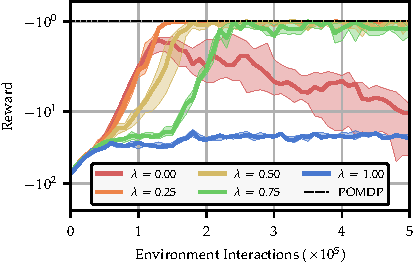
\includegraphics[width=0.95\textwidth]{figures/OSC/lambda_sweep/lam_sweep_results_TigerDoor_True_tests_results_AdaptAsymDagger_cr_logs_lam_sweep_4_.pdf}
        \caption{Reward.}
        \label{fig:osc:lambda:reward}
    \end{subfigure}%
    %
    \hfill%
    %
    \begin{subfigure}[t]{0.48\textwidth}
        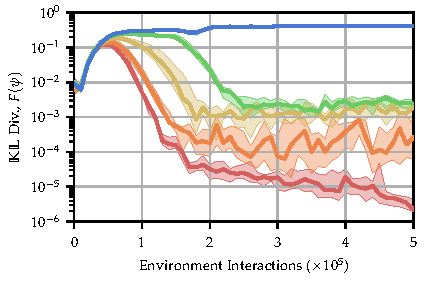
\includegraphics[width=0.95\textwidth]{figures/OSC/lambda_sweep/lam_sweep_divergence_TigerDoor_True_tests_results_AdaptAsymDagger_cr_logs_lam_sweep_4_.pdf}
        \caption{Divergence.}
        \label{fig:osc:lambda:divergence}
    \end{subfigure}%
    \vspace{-0.25cm}
    \caption{Results showing the affect of the GAE parameter $\lambda$ on A2D, applied to the  Tiger Door 2 environment.  The reward is normalized such that the optimal reward under the POMDP is $-10^{0}$.  As predicted, we see that lower $\lambda$ values yield faster convergence and monotonically lower policy divergences.  However, as this is equivalent to TD0, the RL is unstable (obscured in this plot are short, sharp drops in the reward and rises in the divergence).  Eventually, all traces begin to diverge from the optimal policy.  For any $\lambda$ value less than unity, convergence is stable (and the short, sharp drops do not exist).  Finally, and again as predicted, we see that learning does not converge when $\lambda = 1$, with reward remaining flat and low, and the divergence remaining high. { }%
    }
    \label{fig:osc:lambda}
\end{figure}


We note that Frozen Lake subtly exhibits the bias in the Monte Carlo gradient estimator if the value of $\lambda$ is too high.  First, the trainee quickly converges to the optimal partially observing policy (and so the environment \emph{is} solved).   Then, after \emph{many} more optimization steps, the probability that the agent steps onto the ice can rise slightly.  This causes the divergence to rise slightly and the expected stochastic reward to fall slightly before stabilizing.  The rise is small enough that the deterministic policy evaluation remains unchanged.  However, as predicted by the analysis above, this behavior can be eradicated by reducing the value of $\lambda$.  However, in RL generally, lowering $\lambda$ can stall, or even halt, learning from the outset by overreliance on biased function approximators.  This can cause the optimization to become stuck in local minima.  As eluded to above, we find that we can control this behavior by slightly reducing the value of $\lambda$ from its initial value during the optimization.  This minimizes the dependency on function approximators early in training and retains the fast and reliable convergence to the optimal policy, and then attenuates any bias after learning has converged.  While we believe this behavior only presents in a small number of very specific environments and can be eradicated through tuning of hyperparameters, we propose that further investigation of adaptively controlling $\lambda$ during the optimization is a promising and practical future research directions.  More generally, investigating methods for quantifying and ameliorating this bias is an exciting topic of future research.  Note that we did not apply this annealing in the experiments presented in the main text.  When the Q function is estimated, this behavior is not observed, and the reward remains optimal and the divergence remains low.  

It is also paramount to highlight here that A2D, at its core, is underpinned by an RL step, and more specifically, a policy gradient step, and hence all the considerations when designing, applying and tuning a regular RL algorithm still apply in A2D. In fact, A2D can, in many respects, be considered a special class of projected policy gradient methods.  Specifically, we optimize \emph{through} the projection defined by AIL, guaranteeing the desired behavior through subsequent imitation. Therefore, in this respect, it is important to reinforce that A2D does not provide a ``free lunch,'' and hyperparameters are still important and can have direct affects on the performance of A2D -- even if, in practice, we find that A2D works well when using many of the same hyperparameters as RL in the underlying MDP.  

The strong dependency on the Q function leads us to recommend that ``default'' A2D algorithm is to not directly estimate the Q function, and instead estimate the advantage directly from the Monte Carlo trajectories, and the bias is tolerated, or $\lambda$ adjusted accordingly.  There are then two instruments available to diagnose if a Q function must be directly approximated: if there is consistently a performance gap between the expert policy and the agent policy, or, if there is a non-negligible $\mathbb{KL}$ divergence between the expert and agent policy (indicating the policies are not being forced to be identifiable).  If either of these behaviors are observed, then a Q function should be directly estimated.  

While the discussion and example presented in this example provide some explanation of this behavior, we were unable to provide a concrete definition, condition, or test identifying when direct estimation of the Q function is required, or, precise mathematical quantification of how $\lambda$ influences the bias.  Crucially, the core of this behavior is a function of the \emph{environment}, and hence there may be no readily available or easy-to-test condition for when a Q function is required.  Beyond this, this effect may manifest as a complication in any method for ameliorating the drawbacks of AIL, and hence further investigation of this is a challenging, interesting, and potentially pivotal theoretical topic for future research, studying the very nature of MDP and POMDPs.  Beyond this, building further intuition, understanding, and eventually defining, the relative influence of different hyperparameter settings in A2D, particularly between when estimating Q and not estimating Q, is a future research direction with great practical benefits.  


\begin{figure*}[t]

    \begin{subfigure}[t]{0.42\textwidth}
        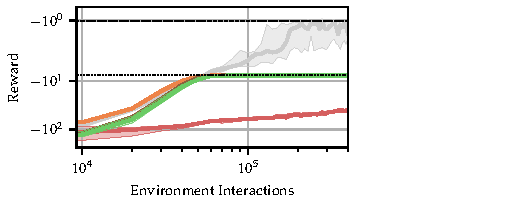
\includegraphics[width=0.95\textwidth]{figures/sec4/cr/lg/sec4_representation_IceLake_True_cr_logs_LavaGap_LavaGapCompiledRun_.pdf}
        \caption{Frozen Lake.}
        \label{supp:fig:grid:a2dplot_2:lg}
    \end{subfigure}%
    %
    \hfill%
    %
    \begin{subfigure}[t]{0.42\textwidth}
        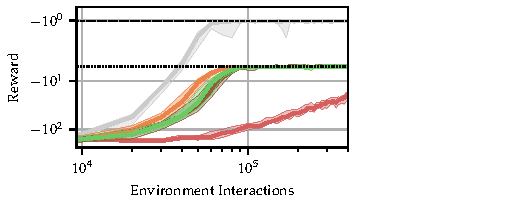
\includegraphics[width=0.95\textwidth]{figures/sec4/cr/td/sec4_representation_TigerDoor_True_cr_logs_TigerDoor_TigerDoorCompiledRun_.pdf}
        \caption{Tiger Door.}
        \label{supp:fig:grid:a2dplot_2:td}
    \end{subfigure}%%
    %
    \hfill%
    %
    \begin{subfigure}[t]{0.15\textwidth}
        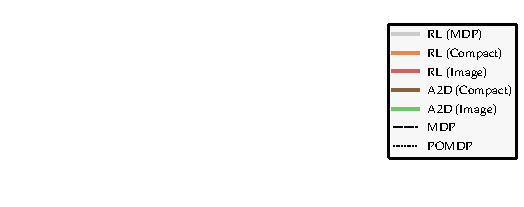
\includegraphics[width=0.95\textwidth]{figures/sec4/legend_representation.pdf}
    \end{subfigure}%

    \caption{Training curves comparing convergence of A2D and vanilla RL on the POMDP for compact (one-hot vector) representations and image-based representations.  We see that RL on the compact partial representation (orange) converges to the optimal POMDP reward (horizontal dotted line, $-9 \times 10^0$ and $-7 \times 10^0$) quickly, and in a sample complexity similar to the best-case convergence of RL in the MDP (gray), which converges to the optimal MDP reward (horizontal dashed line, $- 1 \times 10^0$), when both use hyperparameters comparable to as were used with A2D.  In contrast, RL on the images (red) converges slowly, and does not reach the optimal POMDP reward within the allocated computational budget.  A2D on the other hand converges to the optimal POMDP reward in a sample complexity commensurate with RL operating directly on the compact representation, for \emph{both} image-based and compact representations (brown and green respectively).  This confirms our hypothesis that A2D can reduce the complexity of operating in high-dimensional, partially observed environments to a complexity commensurate with the best-possible convergence rate obtained by performing RL directly on the most efficient encoding or complete state.  { }
    }
    \label{supp:fig:grid:a2dplot_2}
\end{figure*}

\subsection{Differences in Representation}
In Figure \ref{supp:fig:grid:a2dplot_2} we investigate A2D when the trainee uses different representations.  Specifically, we investigate using a compact-but-partial vector representation (labeled as \emph{Compact}), and the original image-based representation (labeled as \emph{Image}).  Both representations include the same partial information, but the compact representation is a much more efficient representation for RL.  The compact representation for Frozen Lake is a length $25$ one-hot vector representing the position of the agent.  For Tiger Door the compact representation is the concatenation of three one-vectors: a length $25$ one-hot vector encoding the position of the agent, a length two vector encoding the position of the goal, and a length two vector encoding the position of the hazard.  The goal and hazard vectors are all zeros until the button is pressed, at which time they become one-hot vectors.  This can be considered as the optimal encoding of the observation and action history.  We note that analytically recovering such an encoding is not always possible (in the AV example, for instance), and learning an encoding (c.f. \emph{Pre-Enc} in Figure \ref{fig:gridworld_asym}) is unreliable, and introduces a non-trivial amount of additional complexity and hyperparameter tuning.  

Results are shown in Figure \ref{supp:fig:grid:a2dplot_2}.  We see performing RL directly on the compact representation (\emph{RL (Compact)}) is fast and stable.  Direct RL in the image-based representation (\emph{RL (Image)}) is slow, and does not converge within the computational budget.  For both Frozen Lake and Tiger Door, A2D converges in a similar number of interactions for both image-based inputs (\emph{A2D (Image)}) and the compact representation (\emph{A2D (Compact)}), and that is commensurate with the convergence of an omniscient MDP expert and RL in the compact state, when using the A2D hyperparameters.  This shows that A2D has successfully abstracted the perception task into the efficient AIL step, and performs RL in the efficient and low-variance omniscient state representation in the best-case sample complexity for those hyperparameters.  This means that A2D is able to exploit the relative strengths of RL to offset the weaknesses of AIL, and vice versa, in an efficient, low-overhead and end-to-end manner.  Crucially, the expert is co-trained with the trainee, and hence there is no requirement for pre-specified expert policies or example trajectories from which to learn policies or static encoders.  


\newpage
